%%%%%%%%%%%%%%%%%%%%%%%%%%%%%%%%%%%%%%%%%%%%%%
% An example of a lab report write-up.
%%%%%%%%%%%%%%%%%%%%%%%%%%%%%%%%%%%%%%%%%%%%%% 
% This is a combination of several labs that I have done in the past for 
% Computer Engineering, so it is not to be taken literally, but instead used as 
% a great starting template for your own lab write up.  When creating this 
% template, I tried to keep in mind all of the functions and functionality of 
% LaTeX that I spent a lot of time researching and using in my lab reports and 
% include them here so that it is fairly easy for students first learning LaTeX
% to jump on in and get immediate results.  However, I do assume that the 
% person using this guide has already created at least a "Hello World" PDF 
% document using LaTeX (which means it's installed and ready to go). 
%
% My preference for developing in LaTeX is to use the LaTeX Plugin for gedit in 
% Linux.  There are others for Mac and Windows as well (particularly MikTeX).  
% Another excellent plugin is the Calc2LaTeX plugin for the OpenOffice suite.  
% It makes it very easy to create a large table very quickly.  
%
% Professors have different tastes for how they want the lab write-ups done, so 
% check with the section layout for your class and create a template file for 
% each class (my recommendation).
%
% Also, there is a list of common commands at the bottom of this document.  Use
% these as a quick reference.  If you'd like more, you can view the "LaTeX Cheat
% Sheet.pdf" included with this template material. 
%
% (c) 2009 Derek R. Hildreth <derek@derekhildreth.com> http://www.derekhildreth.com 
% This work is licensed under the Creative Commons Attribution-NonCommercial-ShareAlike License. To view a copy of this license, visit http://creativecommons.org/licenses/by-nc-sa/1.0/ or send a letter to Creative Commons, 559 Nathan Abbott Way, Stanford, California 94305, USA.
%%%%%%%%%%%%%%%%%%%%%%%%%%%%%%%%%%%%%%%%%%%%%%
\documentclass[aps,letterpaper,10pt]{revtex4}
\input kvmacros % For Karnaugh Maps (K-Maps)

\usepackage{endnotes}
\usepackage{graphicx} % For images
\usepackage{float}    % For tables and other floats
\usepackage{verbatim} % For comments and other
\usepackage{amsmath}  % For math
\usepackage{amssymb}  % For more math
\usepackage{fullpage} % Set margins and place page numbers at bottom center
\usepackage{listings} % For source code
\usepackage{gensymb} %ohms and shit
\usepackage{subfig}   % For subfigures
\usepackage[usenames,dvipsnames]{color} % For colors and names
\usepackage[pdftex]{hyperref}           % For hyperlinks and indexing the PDF
\hypersetup{ % play with the different link colors here
    colorlinks,
    citecolor=blue,
    filecolor=blue,
    linkcolor=blue,
    urlcolor=blue % set to black to prevent printing blue links
}
\usepackage{tikz} \usepackage{circuitikz} \usepackage{siunitx}

\definecolor{mygrey}{gray}{.96} % Light Grey
\lstset{ 
	language=[ISO]C++,              % choose the language of the code ("language=Verilog" is popular as well)
   tabsize=3,							  % sets the size of the tabs in spaces (1 Tab is replaced with 3 spaces)
	basicstyle=\tiny,               % the size of the fonts that are used for the code
	numbers=left,                   % where to put the line-numbers
	numberstyle=\tiny,              % the size of the fonts that are used for the line-numbers
	stepnumber=2,                   % the step between two line-numbers. If it's 1 each line will be numbered
	numbersep=5pt,                  % how far the line-numbers are from the code
	backgroundcolor=\color{mygrey}, % choose the background color. You must add \usepackage{color}
	%showspaces=false,              % show spaces adding particular underscores
	%showstringspaces=false,        % underline spaces within strings
	%showtabs=false,                % show tabs within strings adding particular underscores
	frame=single,	                 % adds a frame around the code
	tabsize=3,	                    % sets default tabsize to 2 spaces
	captionpos=b,                   % sets the caption-position to bottom
	breaklines=true,                % sets automatic line breaking
	breakatwhitespace=false,        % sets if automatic breaks should only happen at whitespace
	%escapeinside={\%*}{*)},        % if you want to add a comment within your code
	commentstyle=\color{BrickRed}   % sets the comment style
}

% Make units a little nicer looking and faster to type
\newcommand{\Hz}{\textsl{Hz}}
\newcommand{\KHz}{\textsl{KHz}}
\newcommand{\MHz}{\textsl{MHz}}
\newcommand{\GHz}{\textsl{GHz}}
\newcommand{\ns}{\textsl{ns}}
\newcommand{\ms}{\textsl{ms}}
\newcommand{\s}{\textsl{s}}

%for ease of entry
\newcommand{\voltage}[1]{$V_{#1}$}
\newcommand{\current}[1]{$I_{#1}$}
\newcommand{\resistance}[1]{$R_{#1}$}
\newcommand{\kiloohm}[1]{\SI{#1}{\kilo\ohm}}
\newcommand{\ohms}[1]{\SI{#1}{\ohm}}

%spacing
%Custom indenting
\newcommand{\single}{\hspace*{0.5cm}}
\newcommand{\double}{\hspace*{1cm}}


% TITLE PAGE CONTENT %%%%%%%%%%%%%%%%%%%%%%%%
% Remember to fill this section out for each
% lab write-up.
%%%%%%%%%%%%%%%%%%%%%%%%%%%%%%%%%%%%%%%%%%%%%
\newcommand{\labname}{EE 119c Functional Specification}
\newcommand{\descript}{FPGA-Based Pitch Detector and Tuner}
\newcommand{\authorname}{Dan Pipe-Mazo}
\newcommand{\professor}{Glen George}
\newcommand{\classno}{Spring 2013}
% END TITLE PAGE CONTENT %%%%%%%%%%%%%%%%%%%%


\begin{document}  % START THE DOCUMENT!


% TITLE PAGE %%%%%%%%%%%%%%%%%%%%%%%%%%%%%%%%%%%%%%
% If you'd like to change the content of this,
% do it in the "TITLE PAGE CONTENT" directly above
% this message
%%%%%%%%%%%%%%%%%%%%%%%%%%%%%%%%%%%%%%%%%%%%%%%%%%%
\begin{titlepage}
\begin{center}
{\LARGE \textsc{\labname:} \\ \vspace{4pt}}
{\Large \textsc{\descript} \\ \vspace{4pt}} 
\rule[13pt]{\textwidth}{1pt} \\ \vspace{150pt}
{\large By: \authorname \\ \vspace{10pt}
Instructor: \professor \\ \vspace{10pt}
California Institute of Technology \\ \vspace{10pt}
\classno \\ \vspace{10pt}}
\end{center}
\end{titlepage}
% END TITLE PAGE %%%%%%%%%%%%%%%%%%%%%%%%%%%%%%%%%%

%%%%%%%%%%%%%%%%%%%%%%%%%%%%%%
%%%%%%%%%%%%%%%%%%%%%%%%%%%%%%
\section{Description}

This project is a digital, real-time pitch detection and tuning system. The system is able to determine the dominant frequency of any audio signal between 50 and 5,000Hz with 2 cent general accuracy. The detected frequency will be displayed in floating-point form on a display with 0.001 Hz resolution. The device can wither be used in a general pitch detection mode, or a string tuning mode in which the performance is tailored to better detect the desired frequency. \\ 

The system uses a variable sampling rate in order to correctly identify frequencies. At the time at which the pitch detection algorithm converges, the sampling rate will be approximately 1024 times the detected frequency. In order to detect frequency, an autocorrelation algorithm is employed. The autocorrelation algorithm begins scanning for the lowest detectable frequency, and increases the sampling rate until the autocorrelation peak lands in the range of acceptable bins for which the accuracy specifications are met. 

The system also has the ability to use a stepper motor to automatically tune a guitar string. The system will run its pitch detection algorithm and attempt to tune the string using the auxiliary stepper motor unit until the pitch detected is within the acceptable accuracy thresholds. 

%%%%%%%%%%%%%%%%%%%%%%%%%%%%%%
%%%%%%%%%%%%%%%%%%%%%%%%%%%%%%
\section{Inputs}

The LM4550 audio codec takes audio input from either a standard carded microphone or a line-level audio signal. This codec then supplies 18-bit PCM samples over a serial connection to the system. \\

The user is able to input commands through the eight on-board switches, five on-board buttons or reset button. \\

A 5V power supply is needed to run the FPGA and all auxiliary devices except for the stepper motor. The stepper motor requires a 30V power supply capable of sourcing at least 0.5A. 

%%%%%%%%%%%%%%%%%%%%%%%%%%%%%%
%%%%%%%%%%%%%%%%%%%%%%%%%%%%%%
\section{Outputs}

The system outputs important information to the 20-character x 4 line LCD dot matrix display.\\

If in automatic tuning mode, the system outputs step and direction commands to an A3967 stepper motor driver which in turn outputs controls to a 0.33A/phase, 200 step/rotation stepper motor which is used to turn the guitar tuning knob. \\

The system also outputs 18-bit PCM audio samples to the LM4550 codec which then outputs an analog audio signal to the headphone out jack on the board. 

%%%%%%%%%%%%%%%%%%%%%%%%%%%%%%
%%%%%%%%%%%%%%%%%%%%%%%%%%%%%%
\section{User Interface}

\textsc{System Modes} \\

The system has 7 basic modes of operation:
\begin{enumerate}
\item \textbf{Free tune mode} Capable of detecting any input frequency between 50 and 5,000 Hz to within 2 cent accuracy
\item \textbf{Tune E2 string mode} Capable of detecting any frequency between 50 and 5,000 Hz. Detects frequencies around 82.407 Hz to within 2 cent accuracy
\item \textbf{Tune A2 string mode} Capable of detecting any frequency between 60 and 5,000 Hz. Detects frequencies around 110.000 Hz to within 2 cent accuracy
\item \textbf{Tune D3 string mode} Capable of detecting any frequency between 80 and 5,000 Hz. Detects frequencies around 146.832 Hz to within 2 cent accuracy
\item \textbf{Tune G3 string mode} Capable of detecting any frequency between 108 and 5,000 Hz. Detects frequencies around 195.998 Hz to within 2 cent accuracy
\item \textbf{Tune B3 string mode} Capable of detecting any frequency between 135 and 5,000 Hz. Detects frequencies around 246.942 Hz to within 2 cent accuracy
\item \textbf{Tune E4 string mode} Capable of detecting any frequency between 182 and 5,000 Hz. Detects frequencies around 329.628 Hz to within 2 cent accuracy
\end{enumerate}

The free tune mode should be used when attempting to identify an unknown frequency within the acceptable range. Each guitar string has its own mode which should be used when attempting to tune that particular string. The free tune mode guarantees accuracy across all frequencies, while the specific string tuning modes are most accurate around the respective string's frequency, though they can detect any frequency in the above range. The tradeoff being made between the free tune modes and the individual string modes is that of consistency. The free tune algorithm can occasionally misidentify overtones or undertones. This behavior is less tolerable when attempting to tune a guitar string, so the algorithm is slightly modified to improve consistency of identifying the correct frequency of interest. \\

\textsc{Pushbuttons} \\

When the system is reset, it will start up in free tune mode. The user may switch through the modes using the left and right buttons on the FPGA board. Pressing the right button will increase the mode as listed above and pressing the left button will decrease the mode. If the right button is pressed in tune E4 string mode, then the system will wrap back around to free tune mode. If the left button is pressed in free tune mode, then the system will wrap back around to tune E4 string mode. \\

When the system is in one of the string tuning modes (any mode other than free tune mode), pressing the middle button will activate automatic tuning mode. This will not engage the motors, but simply put the system into a state where it is ready to run the automatic tuning algorithm using the stepper motor. When the system is in automatic tuning mode, pressing the top button will engage the stepper motor and will run the automatic tuning algorithm. Once this button is pressed, the stepper motor will attempt to turn the tuning knob to tune to the frequency corresponding the the string mode which the system is in. The stepper motor can be disengaged by pressing this button again. Changing between any string mode or turning off automatic tuning mode will also disengage the stepper motor. \\

If the string being tuned reaches the desired frequency, the system will alert the user that the correct tune has been achieved. The bottom pushbutton can be used to dismiss the tuned message and either begin tuning another string or continue to tune the current string. \\

\textsc{Display} \\

The display is split into 4 lines, with 20 characters on each line. \\

The first line of the display shows which mode the system is currently in. \\

The second line of the display shows the target frequency for tuning if the system is in string tuning mode, else it is blank. \\

The third line of the display shows the most recent frequency which the system detected. \\

The fourth line of the display shows status information regarding the state of the tuning algorithm if the system is in string tuning mode, else it is blank. If the frequency detected falls within the accuracy bounds for the current string which the system is attempting to detect, then this line will show the word "tuned". Else, if the system is not in automatic tuning mode, this line will be blank. If the string is not in tune and the system is in automatic tuning mode, then this line will display whether or not the automatic tuning algorithm is running. The state of the automatic tuning algorithm is toggled by pressing the top pushbutton. \\

\textsc{Switches} \\

The switches are numbered from 7 to 0 from left to right on the FPGA board with the pushbutton array in the bottom right corner of the board as you look at it. All switches are considered to be a '1' when in the up position and a '0' in the down position. \\

Switches 7 to 3 (MSB to LSB) make up a 5-bit unsigned word which controls the volume of the output audio at the headphone jack. Volume increases with higher word values.\\

Switch 2 controls the input to the LM4550 audio codec. If this switch is up, then the line in input will be fed into the codec's ADC and will serve as the analog signal for the samples which the system receives. If this switch is down, then the microphone will serve as the input to the codec. \\

Switches 1 and 0 make up the 2-bit codeword which controls the stepping resolution of the stepper motor driver. This switches are fed into the MS2 and MS1 inputs, respectively, of the A3967 stepper motor driver. The values of MS2 and MS1 and corresponding step resolutions can be found in the table below. Best performance is obtained with these switches both in the 'up' position, since this allows the finest stepping control. Quicker convergence can be obtained using full stepping mode, since less steps need to be taken.

\begin{center}
\begin{tabular}{|c|c|c|}
\hline
MS2 & MS1 &  Step Resolution \\
\hline
0 & 0 & Full Step \\
0 & 1 & 1/2 Step \\
1 & 0 & 1/4 Step \\
1 & 1 & 1/8 Step \\
\hline
\end{tabular}
\end{center}

\textsc{Motor} \\

When using the system to automatically tune a guitar string, it is necessary for the user to attach the motor and supplied tuning peg bracket to the guitar for use. To do this, simply hold the motor by the casing and insert the guitar tuning peg into the tuning peg bracket attached to the motor drive shaft. When ready to tune, engage the motor by pressing the top pushbutton. At this point, the system is ready to attempt an automatic tune, so simply strum string until the word "tuned" appears on the bottom line of the display.\\
%%%%%%%%%%%%%%%%%%%%%%%%%%%%%
%%%%%%%%%%%%%%%%%%%%%%%%%%%%%%
\section{Block Diagram}
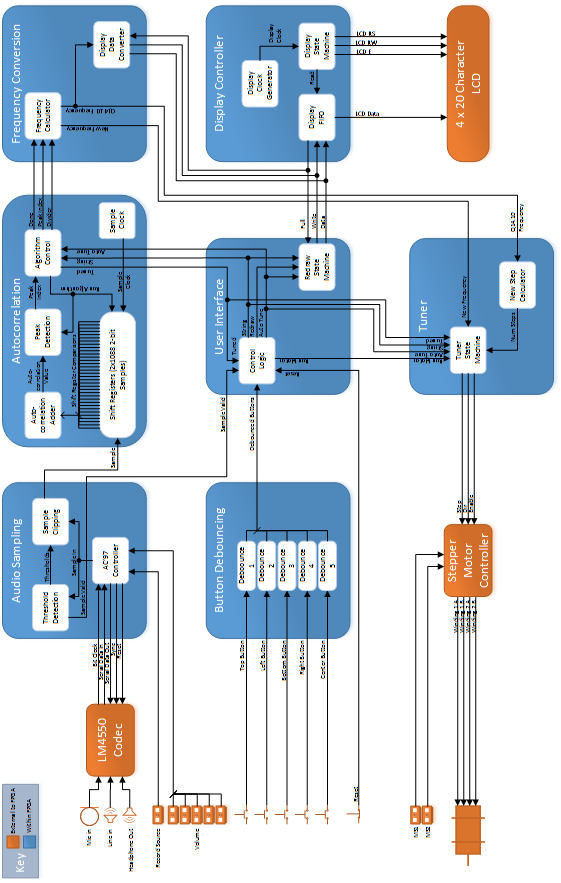
\includegraphics[width=0.9\textwidth]{guitar_tuner_block_diagram.png}

%%%%%%%%%%%%%%%%%%%%%%%%%%%%%
%%%%%%%%%%%%%%%%%%%%%%%%%%%%%%
\section{Block Descriptions}

%%%%%%%%%%%%%%%%%%%%%%%%%%%%%
%%%%%%%%%%%%%%%%%%%%%%%%%%%%%%
\section{Algorithm Description}

Audio samples are input through a standard cardiod microphone to an LM4550 audio codec. This codec uses the AC'97 standard to transmit 18-bit signed PCM samples over serial to the FPGA at  a rate of 48 KHz. Once within the FPGA, the audio samples are decimated from 18 bits to 2 bits. In order to do this, a "thresholding" mechanism is employed. After every 1024 samples, a sample maximum and minimum are identified. The sample amplitude is then calculated as the difference between the maximum and the minimum. Thresholds are then set at
$$ threshold_{high} = maximum - \frac{amplitude}{8}$$ and $$threshold_{low} = mimumum + \frac{amplitude}{8}$$
If the incoming audio sample is greater then the high threshold, it is assigned a value of 1. If the sample is below the minimum threshold, it is assigned a value of -1. If the sample is between the two thresholds, it is assigned a value of 0. This allows for samples to be defined in 2 bits as opposed to 18, and also serves to filter out high frequency noise. \\

The 2-bit samples are then fed into two 1088-sample shift registers. Each round of the pitch detection algorithm takes 2176 samples. For the first half of the samples (samples 0 - 1087), the input audio signal is fed into both shift registers. For the second half of the samples (samples 1088 - 2175), the incoming audio sample is fed into only one of the shift registers. Between each entry in the two shift registers, there is a simple comparator. If the samples at the $i^{th}$ index in each shift register match, then a '1' is outputted, else a '0'. The 1088 comparator outputs are then fed into a 1088-bit adder tree which computes the bit sum. Using this setup, autocorrelation values are computed. The output of the adder tree for each sample, $i$, in the second half (samples 1088 - 2175) corresponds to the discrete autocorrelation value for bin $(i - 1088)$. \\

The system performs peak detection on the autocorrelation results, and remembers the value and bin number of the maximum overall peak across the entire sampling round. At the end of the round, after 2176 samples have been taken, the identified frequency is equal to the sampling frequency divided by the bin number of the result. However, the algorithm does not stop here. Sampling frequencies are generated using a clock divider to divide down the 100MHz system clock. The algorithm converges when the sampling frequency is as close to 1024 times the identified frequency as possible. In oder to accommodate this, after each round of sampling, a new clock divider is calculated as 
$$new~divider = \frac{old~divider \times (bin + 1)}{1024}$$
When the new divider is equal to the old divider, then the algorithm has converged and the frequency is reported as a clock divider and a bin number.\\

Once a frequency has been found, it is converted from the divider and bin number result into a Q14.10 fixed-point result by performing 
$$detected~frequency  = \frac{system~clock}{divider \times bin} = \frac{100MHz}{divider \times bin}$$
This frequency is then converted to its ASCII equivalent and is output to the display. \\

If the system is in automatic tuning mode, the Q14.10 frequency is also sent to the tuning unit. This unit takes the input frequency and calculates the number of steps which are required to tune the string to the desired frequency. The number of steps needed to be taken is calculated as
$$steps = \frac{(previous~steps) \times (expected~freq - actual~freq)}{previous~freq - actual~freq}$$
where "expected freq" is the expected frequency for the string to be in tune, "actual freq" is the new reported frequency from the autocorrelation unit, "previous freq" is the lacteal frequency from the previous tuning attempt and "previous steps" are the number of steps taken in the previous tuning attempt. Using this algorithm, the system dynamically learns the spring constant of the string and converges to the correct frequency. If the tuning algorithm is being run for the first time, a predetermined number of steps are taken. 


%%%%%%%%%%%%%%%%%%%%%%%%%%%%%
%%%%%%%%%%%%%%%%%%%%%%%%%%%%%%
\section{FPGA Size}

The final design utilizes approximately 2,500 Xilinx Spartan 6 standard SLICEs and 30 Xilinx Spartan 6 DSP48A1 slices. Each standard SLICE contains 8 DFFs and four six-input LUTS. Each DSP48A1 slice contains an 18-bit multiplier, an adder and an accumulator. The XTREME-DSP slices are mainly used for the two dividers required by the design. The design was created so that the dividers are not in time-critical sections of the code. They can easily be replaced with subtraction loops, allowing the entire design to be compiled into simple logic and freeing the design from using any FPGA-specific resources. The design also uses 2 8-bit block RAM blocks which are used in a FIFO to communicate between the main control loop and the display controller. 


%%%%%%%%%%%%%%%%%%%%%%%%%%%%%
%%%%%%%%%%%%%%%%%%%%%%%%%%%%%%
\section{Algorithm Runtime}
The algorithm begins by taking 2176 samples at 24.42 KHz, which takes 89.1ms. Each subsequent sample attempt will run significantly faster than 89.1 ms, since this is the slowest possible sampling rate. While the algorithm takes a variable amount of time to converge, it will typically converge between 100 - 200 ms. \\

If the system is in automatic tuning mode, steps are sent at a rate of ~700Hz, with a 200ms wait period after each string of steps before enabling the autocorrelation algorithm to run again. This causes the automatic tuning algorithm to converge on the order of 1 - 5 seconds, depending on how far off the string was from being tuned. 

%%%%%%%%%%%%%%%%%%%%%%%%%%%%%
%%%%%%%%%%%%%%%%%%%%%%%%%%%%%%
\section{Functional Specification}
The FPGA-Based Pitch Detector and Tuner will display the frequency of any audible tone between 50 and 5,000Hz to 2 cent accuracy. 

\noindent \textsc{\large Features}\\

\begin{itemize}
\item LCD Display shows detected frequency, closest musical note and margin of error from closest musical note. 
\item FPGA-based sigma-delta converter sampling at speeds up to 50Msps.
\item Frequency identification accuracy within 1Hz and 0.1\% for all values between 15Hz and 5000Hz ( $C_0$ to $D^\#_8$).
\item Stepper motor with 200 steps per revolution and micro stepping capability allows for precision tuning while also having enough torque to crank stiff tuning knobs. 
\item Precise, digitally-controlled amplification and background-noise cancellation prevents erroneous output from displaying on the screen and increases the accuracy of the system.
\end{itemize}

\noindent \textsc{\large Inputs}\\

\begin{itemize}
\item Pushbutton rotary encoder and four input keys (up, down, left, right) for navigating through the menus and features of the user interface
\item Microphone to capture audio
\end{itemize}

\noindent \textsc{\large Outputs}\\

\begin{itemize}
\item LCD screen displays exact frequency of tone played, closest note, and margin of error from closest note
\item If automatic tuning is activated, stepper motor will rotate to tune instrument
\end{itemize}

\noindent \textsc{\large Major Hardware}\\

The FPGA-Based pitch detector and Tuner will run on a Xilinx FPGA. The FPGA will need to be between 2 million and 4 million gates, as discussed in the FPGA Size Estimate section above. \\

In addition to the FPGA, the pitch detector will utilize:
\begin{itemize}
\item A sigma-delta converter with $\geq 20$ bits of resolution capable of sampling at speeds greater than 50Msps. 
\item An analog low-pass filter (10KHz corner frequency), in order to allow for faster pitch calculation times. 
\item Analog voltage subtractor and amplifying circuitry controlled by digital potentiometers in order to subtract out background noise and perform clipping. 
\item A LCD or similar display.
\item A stepper motor with $\geq 200$ steps per revolution, accompanied by stepper motor driver chips. 
\end{itemize}

\noindent \textsc{\large User Interface}\\

The FPGA-Based Pitch Detector and tuner will feature a LCD which the act to both display information to the user and take input from the user. The LCD and accompanying switches and rotary encoder will allow the user to select a mode to operate the device in from one of the following modes:
\begin{enumerate}
\item \textbf{General Pitch Detection}: Have the pitch detector continuously run and display the current pitch of audio input. Pitch shown in to an appropriate number of decimal places. 
\item \textbf{Tuning}: Choose a note in the range of  $C_0$ to $D^\#_8$ and view how close to in tune the audio input is to the desired note. Real-time feedback allows for easy and quick manual tuning. Pitch shown in Hz to an appropriate number of decimal places. Visual feedback as to how far out of tune from the desired note is provided on-screen.
\item \textbf{Automatic Tuning}: For any open-string guitar tuning, choose a note, attach the stepper motor unit to the tuning knob, pluck the note once, and by the time time note finishes playing, it will be perfectly in tune. 
\end{enumerate}

\noindent \textsc{\large Limitations}\\

Current limitations for the device are:
\begin{itemize}
\item Can only detect frequencies from 15Hz to 5KHz within 0.1\% and 1Hz error margins
\item Automatic tuning only works for guitars
\item Not able to detect multiple notes being played at the same time
\end{itemize}
All of the above limitations can potentially be solved through further development, but are not included in the base design of the project. 

\newpage
\section{Block Diagram}
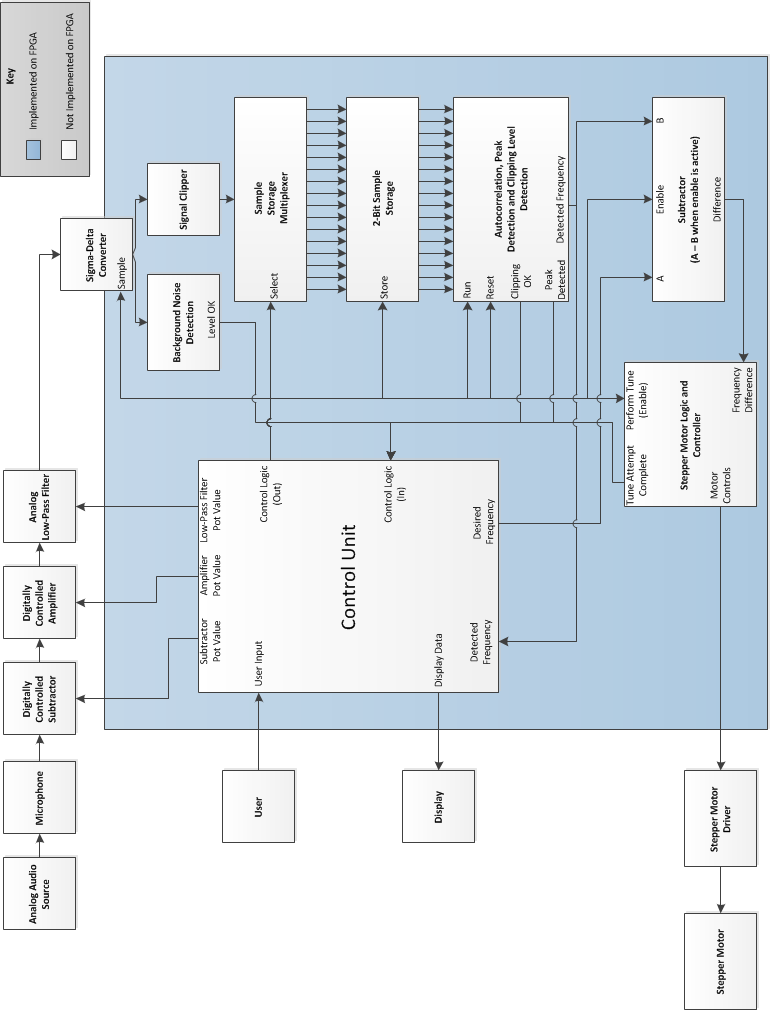
\includegraphics[width=\textwidth]{EE119c_block_diagram.png}


\section{Demonstration}
The project will be demonstrated with the following tests:
\begin{enumerate}
\item Use a function generator to generate tones in the range of 15 to 5000 Hz, and view the display of the pitch detector to verify functionality. Ensure that 1Hz or 0.1\% error margins are obeyed, whichever margin is tighter. 
\item Use a function generator to generate tones close to but not exactly that of E2, A2, D3, G3, B3 and E4, the 6 open strings of the guitar, and use the information on the LCD of the pitch detector to manually tune the function generator to precise frequencies. 
\item Untune a guitar string and use the pitch detector's automatic tuning motor to automatically tune the string in a single pluck.
\end{enumerate}

\section{Schedule}
Weekly milestones are proposed as follows:
\begin{enumerate}
\item Choose all hardware and order/sample parts. Completely flesh out block diagrams, detailing all signals and control logic.
\item Write control unit VHDL code
\item Write sampling and sigma-delta code, breadboard analog circuitry
\item Write autocorrelation and peak detection code
\item Write motor control code, breadboard entire design
\item Integrate all code together, design any PCBs needed
\item Write VHDL test bench
\item Test using test bench and fix bugs
\item Assemble PCBs and final hardware design, more testing and debugging
\item Final testing, presentation and documentation
\end{enumerate}
%%%%%%%%%%%%%%%%%%%%%%%%%%%%%%
%%%%%%%%%%%%%%%%%%%%%%%%%%%%%%
	


%%%%%%%%%%%%%%%%%%%%%%%%%%%%%%
%%%%%%%%%%%%%%%%%%%%%%%%%%%%%


%%%%%%%%%%%%%%%%%%%%%%%%%%%%%%
%%%%%%%%%%%%%%%%%%%%%%%%%%%%%%

\theendnotes
\end{document} % DONE WITH DOCUMENT!


%%%%%%%%%%
PERSONAL FAVORITE LAB WRITE-UP STRUCTURE
%%%%%%%%%%
\section{Introduction}
	% No Text Here
	\subsection{Purpose}
		% Lab objective
	\subsection{Equipment}
		% Any and all equipment used (specific!)
	\subsection{Procedure}
		% Overview of the procedure taken (not-so-specific!)
\newpage
\section{Schematic Diagrams}
	% Any schematics, screenshots, block
   % diagrams used.  Possibly photos or
	% images could go here as well.
\newpage
\section{Experiment Data}
	% Depending on lab, program code would be 
	% included here without the Estimated and 
	% Actual Results.
	\subsection{Estimated Results}
		% Calculated. What it should be.
	\subsection{Actual Results}
		% Measured.  What it actually was.
\newpage
\section{Discussion \& Conclusion}
	% 3 Paragraphs:
		% Restate the objective of the lab
		% Discuss personal trials, errors, and difficulties
		% Conclude the lab


%%%%%%%%%%%%%%%%
COMMON COMMANDS:
%%%%%%%%%%%%%%%%
% IMAGES
begin{figure}[H]
   \begin{center}
      \includegraphics[width=0.6\textwidth]{RTL_SCHEM.png}
   \end{center}
\caption{A screenshot of the RTL Schematics produced from the Verilog code.}
\label{RTL}
\end{figure}

% SUBFIGURES IMAGES
\begin{figure}[H]
  \centering
  \subfloat[LED4 Period]{\label{fig:Per4}\includegraphics[width=0.4\textwidth]{period_led4.png}} \\                
  \subfloat[LED5 Period]{\label{fig:Per5}\includegraphics[width=0.4\textwidth]{period_led5.png}}
  \subfloat[LED6 Period]{\label{fig:Per6}\includegraphics[width=0.4\textwidth]{period_led6.png}}
  \caption{Period of LED blink rate captured by osciliscope.}
  \label{fig:oscil}
\end{figure}

% INSERT SOURCE CODE
\lstset{language=Verilog, tabsize=3, backgroundcolor=\color{mygrey}, basicstyle=\small, commentstyle=\color{BrickRed}}
\lstinputlisting{MODULE.v}

% TEXT TABLE
\begin{table}
\begin{center}
\begin{tabular}{|l|c|c|l|}
	x & x & x & x \\ \hline
	x & x & x & x \\
	x & x & x & x \\ \hline
\end{tabular}
\caption{Caption}
\label{label}
\end{center}
\end{table}

% MATHMATICAL ENVIRONMENT
$ 8 = 2 \times 4 $

% CENTERED FORMULA
\[  \]

% NUMBERED EQUATION
\begin{equation}
	
\end{equation}

% ARRAY OF EQUATIONS (The splat supresses the numbering)
\begin{align*}
	
\end{align*}

% NUMBERED ARRAY OF EQUATIONS
\begin{align}
	
\end{align}

% ACCENTS
\dot{x} % dot
\ddot{x} % double dot
\bar{x} % bar
\tilde{x} % tilde
\vec{x} % vector
\hat{x} % hat
\acute{x} % acute
\grave{x} % grave
\breve{x} % breve
\check{x} % dot (cowboy hat)

% FONTS
\mathrm{text} % roman
\mathsf{text} % sans serif
\mathtt{text} % Typewriter
\mathbb{text} % Blackboard bold
\mathcal{text} % Caligraphy
\mathfrak{text} % Fraktur

\textbf{text} % bold
\textit{text} % italic
\textsl{text} % slanted
\textsc{text} % small caps
\texttt{text} % typewriter
\underline{text} % underline
\emph{text} % emphasized

\begin{tiny}text\end{tiny} % Tiny
\begin{scriptsize}text\end{scriptsize} % Script Size
\begin{footnotesize}text\end{footnotesize} % Footnote Size
\begin{small}text\end{small} % Small
\begin{normalsize}text\end{normalsize} % Normal Size
\begin{large}text\end{large} % Large
\begin{Large}text\end{Large} % Larger
\begin{LARGE}text\end{LARGE} % Very Large
\begin{huge}text\end{huge}   % Huge
\begin{Huge}text\end{Huge}   % Very Huge


% GENERATE TABLE OF CONTENTS AND/OR TABLE OF FIGURES
% These seem to have some issues with the "revtex4" document class.  To use, change
% the very first line of this document to "article" like this:
% \documentclass[aps,letterpaper,10pt]{article}
\tableofcontents
\listoffigures
\listoftables

% INCLUDE A HYPERLINK OR URL
\url{http://www.derekhildreth.com}
\href{http://www.derekhildreth.com}{Derek Hildreth's Website}

% FOR MORE, REFER TO THE "LINUX CHEAT SHEET.PDF" FILE INCLUDED!
